% =============================================================================
% MTH407 Term Project — Technical Interpretation (Rough Draft, English)
%
% Compile with:
%     cd docs && pdflatex report.tex
% or upload report.tex (with the figures path resolved) to Overleaf.
%
% Figures are read from ../output/figures/ via \graphicspath. If you move this
% file, update that line.
% =============================================================================

\documentclass[11pt,a4paper]{article}

% --- Packages ----------------------------------------------------------------
\usepackage[T1]{fontenc}
\usepackage[utf8]{inputenc}
\usepackage[english]{babel}
\usepackage[margin=1in]{geometry}
\usepackage{amsmath,amssymb,amsthm}
\usepackage{graphicx}
\usepackage{booktabs}
\usepackage{caption}
\usepackage{subcaption}
\usepackage{microtype}
\usepackage{xcolor}
\usepackage{enumitem}
\usepackage[colorlinks=true,linkcolor=blue!50!black,urlcolor=blue!50!black,citecolor=blue!50!black]{hyperref}
\usepackage{xurl}
\usepackage{listings}

\graphicspath{{../output/figures/}}

% --- Math shortcuts ----------------------------------------------------------
\newcommand{\R}{\mathbb{R}}
\newcommand{\E}{\mathbb{E}}
\newcommand{\norm}[1]{\left\lVert #1 \right\rVert}
\newcommand{\transpose}{{}^{\mathsf{T}}}
\DeclareMathOperator{\diag}{diag}
\DeclareMathOperator{\trace}{tr}

% =============================================================================
\title{Multi-Sensor TOA-Based 2D Target Localization and Tracking\\
       \large A Technical Interpretation of the MTH407 Term Project}
\author{Ömer Selçuk \\ \texttt{omrselcuk@icloud.com}}
\date{May 2026 \quad\textit{rough draft}}

\begin{document}
\maketitle

% =============================================================================
\begin{abstract}
We design, implement, and analyze a 2D target tracking system that fuses
time-of-arrival (TOA) measurements from $N \in \{2,3,4\}$ stationary sensors
with known positions. A least-squares (LSE) position estimator initializes an
Extended Kalman Filter built on a constant-velocity (CV) motion model with
white-acceleration process noise. We sweep six \emph{(sensor count, geometry)}
cells spanning favorable and degraded configurations, run a 100-trial Monte
Carlo per cell, decompose the position RMSE into smooth-segment and
turn-window components, and run two stress tests: a study of the warm-start
prior's role in the $N{=}3$ collinear ambiguity, and a $\sigma_a$ sensitivity
sweep that exposes the CV-EKF's process-noise tuning trade-off. The results
confirm the expected geometry-dilution scaling
($\text{RMSE} \sim \sigma_r / \sqrt{N}$) on smooth segments, identify
unmodelled-maneuver lag as the dominant contributor to the blended RMSE
metric, and demonstrate that the apparent robustness of the collinear
geometry in the default configuration is wholly due to the warm-start prior
breaking the mirror-image symmetry.
\end{abstract}

% =============================================================================
\section{Introduction}

The course specification (MTH407 dönem projesi) requires a 2D surveillance
system in which time-based measurements from multiple known-position sensors
are used to estimate and track the position of a moving target.  The three
required components are: a measurement-domain simulator (TOA or TDOA), an
LSE-based estimator that produces an initial state vector and covariance, and
an EKF-based tracker.  The required deliverable is an analysis of how
\emph{sensor geometry} affects tracking accuracy.

This report describes the choices made and the resulting performance.  Among
the spec's options we use the TOA model rather than TDOA, fix the target
trajectory to a constant-speed zig-zag with four sharp heading changes,
exercise six geometry cells (two configurations each at $N \in \{2,3,4\}$),
and quantify performance both deterministically and via a 100-trial Monte
Carlo per cell.  Beyond the basic comparison we add two analyses that the
results suggested were necessary: a stress test of the $N{=}3$ collinear
ambiguity, and a sensitivity sweep of the EKF's process-noise tuning
parameter $\sigma_a$.

\paragraph{Implementation.}
The full pipeline is implemented in Python (NumPy / SciPy / Matplotlib) and
distributed as the public repository
\url{https://github.com/selcuko/mth407-toa-target-tracking}.  All figures and
tables in this document are reproduced from the Monte Carlo runs in that
repository.

% =============================================================================
\section{System Model}
\label{sec:system}

\subsection{Geometry and Notation}

Sensors $i = 1, \dots, N$ have known stationary positions
$\mathbf{s}_i \in \R^2$.  The target has unknown position $\mathbf{p}^k \in \R^2$
and velocity $\mathbf{v}^k \in \R^2$ at discrete time $t_k = k T$, with
sample period $T = 0.5\,\mathrm{s}$.  We collect the kinematic state into
$\mathbf{x}^k = \begin{bmatrix} \mathbf{p}^k\transpose & \mathbf{v}^k\transpose \end{bmatrix}\transpose \in \R^4$.

The surveillance area is a $10\,\mathrm{km} \times 10\,\mathrm{km}$ square,
the target speed is fixed at $\norm{\mathbf{v}^k} = 100\,\mathrm{m/s}$, and
the simulation runs for $60\,\mathrm{s}$, yielding $K = 121$ time steps.

\subsection{Ground-Truth Trajectory}

The ground-truth trajectory is a five-leg, constant-speed, piecewise-linear
zig-zag with heading sequence $\theta = (30^\circ, -30^\circ, 50^\circ,
-50^\circ, 30^\circ)$ and starting point $(2000, 5000)\,\mathrm{m}$.  Each
leg lasts $12\,\mathrm{s}$ ($24$ steps), so heading changes occur at steps
$\{24, 48, 72, 96\}$.  These four turns are the core difficulty for the
tracker: the EKF's CV motion model treats them as instantaneous,
unmodelled accelerations.

\subsection{TOA Measurement Model}

Each sensor records the arrival time $z_i^k$ of a signal emitted by the
target at the known time $t_k$:
\begin{equation}
  z_i^k = t_k + \frac{\norm{\mathbf{p}^k - \mathbf{s}_i}}{c} + n_i^k,
  \qquad n_i^k \sim \mathcal{N}(0, \sigma_t^2),
  \label{eq:toa}
\end{equation}
with signal speed $c = 3 \cdot 10^8\,\mathrm{m/s}$ and time-measurement
standard deviation $\sigma_t = 10^{-8}\,\mathrm{s}$.  Internally we simulate
the additive noise in the time domain, faithful to the physics, and convert
to the \emph{range domain} only at the LSE/EKF boundary:
\begin{equation}
  r_i^k \;=\; c \,(z_i^k - t_k)
  \;=\; \norm{\mathbf{p}^k - \mathbf{s}_i} + \nu_i^k,
  \qquad \nu_i^k \sim \mathcal{N}(0, \sigma_r^2),
  \label{eq:range}
\end{equation}
with effective range-noise standard deviation $\sigma_r = c\sigma_t =
3\,\mathrm{m}$.  The measurement noise is independent across sensors and
across time, so the per-step measurement covariance is
$\mathbf{R} = \sigma_r^2 \mathbf{I}_N$.

\paragraph{Why simulate in the time domain.}
Adding range-domain noise directly would give the same numerical result for
a single linear conversion, but framing the simulator in the time domain
preserves the physical interpretation and makes future extensions (clock
biases, asynchronous sensors, TDOA) straightforward.

\subsection{Target Dynamics (CV Model)}

For the EKF we adopt a constant-velocity model in 2D:
\begin{equation}
  \mathbf{x}^{k+1} \;=\; \mathbf{F}(T)\, \mathbf{x}^k + \mathbf{w}^k,
  \qquad \mathbf{w}^k \sim \mathcal{N}(\mathbf{0}, \mathbf{Q}),
\end{equation}
with
\begin{equation}
  \mathbf{F}(T) =
  \begin{bmatrix}
    \mathbf{I}_2 & T \mathbf{I}_2 \\
    \mathbf{0}    & \mathbf{I}_2
  \end{bmatrix},
  \qquad
  \mathbf{Q} \;=\; \sigma_a^2
  \begin{bmatrix}
    \tfrac{T^4}{4}\mathbf{I}_2 & \tfrac{T^3}{2}\mathbf{I}_2 \\[2pt]
    \tfrac{T^3}{2}\mathbf{I}_2 & T^2 \mathbf{I}_2
  \end{bmatrix}.
  \label{eq:cv-Q}
\end{equation}
The discrete white-acceleration form of $\mathbf{Q}$ models the velocity as
a continuous-time random walk; $\sigma_a$ has units of acceleration
($\mathrm{m/s^2}$) and quantifies how much velocity change between samples
the filter is willing to absorb.  We use $\sigma_a = 10\,\mathrm{m/s^2}$ by
default and study the effect of varying it in
\S\ref{sec:sigma-a-sweep}.  Sharp heading changes in the ground-truth
trajectory are \emph{not} explicitly modelled; they are absorbed by the
process noise term and produce transient prediction errors that are the
main story of \S\ref{sec:smooth-vs-turn}.

% =============================================================================
\section{Estimators}
\label{sec:estimators}

\subsection{Least-Squares Position Estimation ($N \ge 3$)}

For $N \ge 3$ sensors the per-step position estimator is iterative
Gauss-Newton on the non-linear range residual.  Stack the $N$ range
measurements at step $k$ as $\mathbf{r}^k \in \R^N$; the residual at iterate
$\mathbf{p}^{(j)}$ is
\begin{equation}
  \boldsymbol{\rho}(\mathbf{p}^{(j)})
  \;=\; \mathbf{r}^k - \mathbf{h}(\mathbf{p}^{(j)}),
  \qquad
  h_i(\mathbf{p}) = \norm{\mathbf{p} - \mathbf{s}_i},
\end{equation}
and the Jacobian of $\mathbf{h}$ is
\begin{equation}
  \mathbf{H}(\mathbf{p}) = \begin{bmatrix} \mathbf{u}_1\transpose \\ \vdots \\ \mathbf{u}_N\transpose \end{bmatrix},
  \qquad
  \mathbf{u}_i \;=\; \frac{\mathbf{p} - \mathbf{s}_i}{\norm{\mathbf{p} - \mathbf{s}_i}}.
  \label{eq:H-rows}
\end{equation}
That is, the $i$-th row of $\mathbf{H}$ is the unit line-of-sight vector
from sensor $i$ to the target.  The Gauss-Newton step is
\begin{equation}
  \mathbf{p}^{(j+1)}
  \;=\; \mathbf{p}^{(j)} + (\mathbf{H}\transpose \mathbf{H})^{-1}
        \mathbf{H}\transpose
        \boldsymbol{\rho}(\mathbf{p}^{(j)}),
\end{equation}
with $\mathbf{H}^+$ used in place of $(\mathbf{H}\transpose
\mathbf{H})^{-1}\mathbf{H}\transpose$ when the latter is ill-conditioned
(this is the case the collinear geometry is supposed to expose).  The
iteration is initialised either at the centroid of the sensors (cold start)
or at the previous step's estimate (warm start), and terminates when
$\norm{\Delta\mathbf{p}} < 10^{-3}\,\mathrm{m}$ or after 30 iterations.

After convergence, the position covariance is approximated by the local
Cram\'er--Rao--style bound
\begin{equation}
  \mathbf{P}_p \;=\; \sigma_r^2 \,(\mathbf{H}\transpose \mathbf{H})^{-1},
  \label{eq:Pp}
\end{equation}
evaluated at the estimate.  Equation~\eqref{eq:Pp} makes the
\emph{geometric dilution of precision} (GDOP) explicit: the smaller the
spread of the unit vectors $\mathbf{u}_i$, the worse-conditioned
$\mathbf{H}\transpose \mathbf{H}$ becomes, and the larger the position
uncertainty for the same per-range $\sigma_r$.

\subsection{LSE for $N = 2$ (Two-Circle Intersection)}

For $N = 2$ the range residuals over-determine no parameters; instead the
two range constraints define two circles, which intersect in $\{0,1,2\}$
points.  Let $d = \norm{\mathbf{s}_2 - \mathbf{s}_1}$ and define
$\mathbf{e}_x = (\mathbf{s}_2 - \mathbf{s}_1)/d$ and a
right-handed perpendicular $\mathbf{e}_y$.  Define
\begin{equation}
  a = \frac{r_1^2 - r_2^2 + d^2}{2d},
  \qquad
  h = \sqrt{\max\!\bigl(r_1^2 - a^2,\, 0\bigr)}.
\end{equation}
The two candidate intersections are
$\mathbf{p}_\pm = \mathbf{s}_1 + a\mathbf{e}_x \pm h\mathbf{e}_y$.
We pick the one closer to a coarse prior $\mathbf{p}_{\text{prior}}$
(provided externally, e.g.\ from rough operational knowledge of the target's
expected start region).  The covariance is approximated by~\eqref{eq:Pp}
evaluated at the chosen candidate.  This estimator is fundamentally
ambiguous and depends on the prior; the analogous degeneracy for $N{=}3$
collinear is the subject of \S\ref{sec:collinear}.

\subsection{State-Vector Initialization}

The initial 4-D state $\hat{\mathbf{x}}_0$ is constructed from LSE position
estimates at the first two time steps:
\begin{equation}
  \hat{\mathbf{p}}_0 = \mathrm{LSE}(\mathbf{r}^0),
  \quad
  \hat{\mathbf{p}}_1 = \mathrm{LSE}(\mathbf{r}^1),
  \quad
  \hat{\mathbf{v}}_0 = \frac{\hat{\mathbf{p}}_1 - \hat{\mathbf{p}}_0}{T}.
\end{equation}
The covariance $\mathbf{P}_0$ inherits position-block from~\eqref{eq:Pp},
the velocity block from finite-difference propagation
$\mathbf{P}_v \approx (\mathbf{P}_{p,0} + \mathbf{P}_{p,1})/T^2$, and the
position--velocity cross-block from
$\mathbf{P}_{pv} \approx -\mathbf{P}_{p,0}/T$, which follows from
$\mathrm{cov}(\hat{\mathbf{p}}_0, \hat{\mathbf{v}}_0) =
-\mathrm{cov}(\hat{\mathbf{p}}_0,\hat{\mathbf{p}}_0)/T$ when $\mathbf{r}^0$
and $\mathbf{r}^1$ are independent.

\subsection{Constant-Velocity Extended Kalman Filter}
\label{subsec:ekf}

The EKF runs the standard predict/update loop with the CV model
\eqref{eq:cv-Q} and the per-sensor range measurement~\eqref{eq:range}.  The
prediction is
\begin{equation}
  \hat{\mathbf{x}}^{k|k-1} = \mathbf{F}\, \hat{\mathbf{x}}^{k-1|k-1},
  \qquad
  \mathbf{P}^{k|k-1} = \mathbf{F}\,\mathbf{P}^{k-1|k-1} \mathbf{F}\transpose + \mathbf{Q}.
\end{equation}
For the update we stack all $N$ range innovations into a single vector and
form the $(N\times 4)$ Jacobian by extending each row of \eqref{eq:H-rows}
with two zeros (since the range function does not depend on velocity):
\begin{equation}
  \mathbf{H}^k \;=\;
  \begin{bmatrix}
    \mathbf{u}_1\transpose & \mathbf{0}_{1\times 2} \\
    \vdots & \vdots \\
    \mathbf{u}_N\transpose & \mathbf{0}_{1\times 2}
  \end{bmatrix},
  \quad
  \mathbf{u}_i \;=\; \frac{\hat{\mathbf{p}}^{k|k-1} - \mathbf{s}_i}
                          {\norm{\hat{\mathbf{p}}^{k|k-1} - \mathbf{s}_i}}.
\end{equation}
The Kalman gain and Joseph-form covariance update are
\begin{align}
  \mathbf{S}^k &= \mathbf{H}^k \mathbf{P}^{k|k-1} (\mathbf{H}^k)\transpose + \mathbf{R}, \\
  \mathbf{K}^k &= \mathbf{P}^{k|k-1} (\mathbf{H}^k)\transpose (\mathbf{S}^k)^{-1}, \\
  \hat{\mathbf{x}}^{k|k} &= \hat{\mathbf{x}}^{k|k-1} + \mathbf{K}^k (\mathbf{r}^k - \mathbf{h}(\hat{\mathbf{p}}^{k|k-1})), \\
  \mathbf{P}^{k|k} &= (\mathbf{I} - \mathbf{K}^k \mathbf{H}^k)\, \mathbf{P}^{k|k-1}\, (\mathbf{I} - \mathbf{K}^k \mathbf{H}^k)\transpose
                    + \mathbf{K}^k \mathbf{R} (\mathbf{K}^k)\transpose.
\end{align}
We use the symmetric Joseph form for numerical stability against
floating-point loss of positive-semidefiniteness.

% =============================================================================
\section{Experimental Setup}

\subsection{Sensor Geometries}

Six (\,$N$, geometry\,) cells are evaluated, designed to span favorable and
degraded configurations at each $N$:

\begin{table}[h]
\centering
\caption{Sensor configurations evaluated.  Coordinates in metres, arena
$10\,\mathrm{km} \times 10\,\mathrm{km}$.}
\label{tab:geometries}
\begin{tabular}{l l l}
\toprule
\textbf{Cell} & \textbf{Description} & \textbf{Sensor positions} \\
\midrule
\texttt{N2\_wide}      & widely separated baseline & $(0,0),\,(10000,10000)$ \\
\texttt{N2\_close}     & close pair on one edge    & $(0,5000),\,(500,5000)$ \\
\texttt{N3\_triangle}  & equilateral around centre & three points on a circle, $r{=}5000$ \\
\texttt{N3\_collinear} & sensors on the line $y{=}0$ & $(1000,0),\,(5000,0),\,(9000,0)$ \\
\texttt{N4\_square}    & arena corners              & $(0,0),(10000,0),(10000,10000),(0,10000)$ \\
\texttt{N4\_cluster}   & corner cluster, $500$\,m   & $(0,0),(500,0),(0,500),(500,500)$ \\
\bottomrule
\end{tabular}
\end{table}

\subsection{Monte Carlo Protocol}

For each cell we run $100$ independent trials, each with a fresh noise
realization (seed $1000+i$ for trial $i$).  The ground-truth trajectory and
sensor positions are identical across trials; only the noise samples
$\{n_i^k\}$ differ.  Per-trial position errors $e^k = \norm{\hat{\mathbf{p}}^k - \mathbf{p}^k}$ are recorded for both the per-step LSE estimator and the
EKF.  RMSE is computed in three buckets:

\begin{description}[leftmargin=2.5em]
  \item[Overall.] Steps $5$ through $K-1$ (skipping the initial filter
        warmup transient).
  \item[Smooth.] Overall mask intersected with the complement of a
        $4$-step turn window after each heading change.
  \item[Turn.] The union of the $4$-step turn windows after each of the
        four heading changes.
\end{description}

This decomposition is essential: the overall RMSE blends two qualitatively
different regimes and obscures the noise-floor performance.

% =============================================================================
\section{Results}
\label{sec:results}

\subsection{Baseline ($N{=}4$ Square)}

Fig.~\ref{fig:baseline} shows the canonical run on the $N{=}4$ square cell
with seed $42$.  The full-arena view confirms that the LSE per-step and EKF
trajectories both follow the ground-truth zig-zag.  The error vs.\ time plot
clearly shows the four spikes at the heading changes and the otherwise
flat baseline.

\begin{figure}[h]
\centering
\begin{subfigure}{0.48\textwidth}
  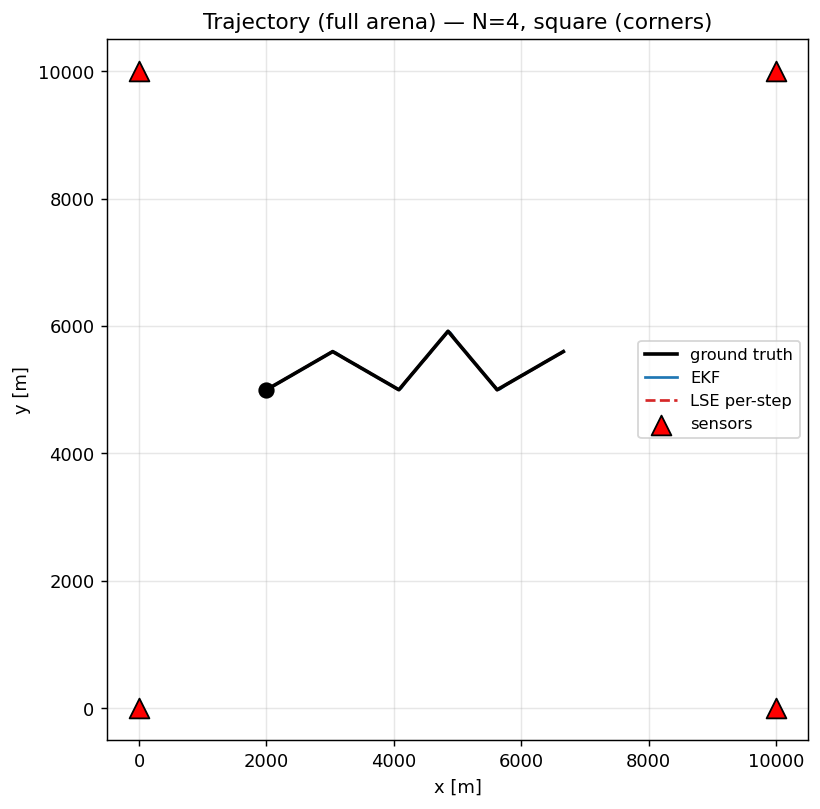
\includegraphics[width=\linewidth]{baseline_N4_square_arena.png}
  \caption{Trajectory in the full $10{\times}10\,\mathrm{km}$ arena.}
\end{subfigure}\hfill
\begin{subfigure}{0.48\textwidth}
  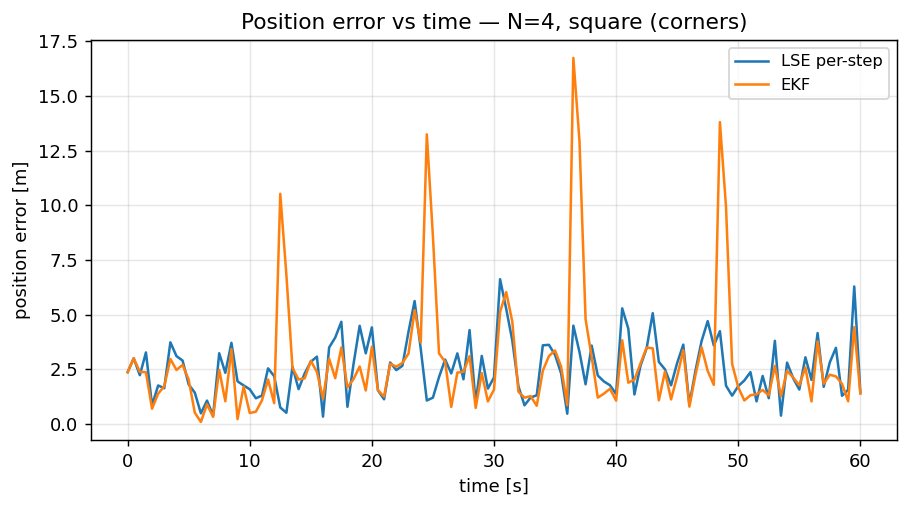
\includegraphics[width=\linewidth]{baseline_N4_square_rmse.png}
  \caption{Position error vs.\ time (single deterministic run).}
\end{subfigure}
\caption{Baseline run on the $N{=}4$ square geometry, seed $42$,
$\sigma_a = 10\,\mathrm{m/s^2}$.}
\label{fig:baseline}
\end{figure}

\subsection{Geometry Sweep --- Monte Carlo Summary}

Table~\ref{tab:mc} gives the 100-trial RMSE summary for the EKF in each of
the six cells, decomposed into smooth-segment and turn-window components.
Fig.~\ref{fig:mc-summary} shows the corresponding bar chart against the
$\sigma_r/\sqrt{N}$ theoretical bound.

\begin{table}[h]
\centering
\caption{EKF position RMSE, 100-trial Monte Carlo, mean $\pm$ standard
deviation across trials. ``Smooth'' excludes the warmup and a 4-step
window after each of the four heading changes; ``Turn'' is the union of
those windows.}
\label{tab:mc}
\begin{tabular}{l r r r}
\toprule
\textbf{Cell} & \textbf{Overall [m]} & \textbf{Smooth [m]} & \textbf{Turn [m]} \\
\midrule
N=2, widespread (corners)   & $28.37 \pm 3.57$    & $26.33 \pm 4.26$   & $38.29 \pm 3.91$  \\
N=2, close pair             & $605.00 \pm 194.11$ & $589.75 \pm 190.11$ & $691.44 \pm 221.63$ \\
N=3, equilateral triangle   & $4.76 \pm 0.18$     & $2.92 \pm 0.17$    & $10.54 \pm 0.57$  \\
N=3, collinear              & $4.48 \pm 0.18$     & $3.28 \pm 0.22$    & $8.84 \pm 0.46$   \\
N=4, square (corners)       & $4.10 \pm 0.17$     & $2.52 \pm 0.13$    & $9.07 \pm 0.51$   \\
N=4, clustered              & $38.95 \pm 3.84$    & $36.90 \pm 3.92$   & $49.55 \pm 6.60$  \\
\bottomrule
\end{tabular}
\end{table}

\begin{figure}[h]
\centering
\begin{subfigure}{0.49\textwidth}
  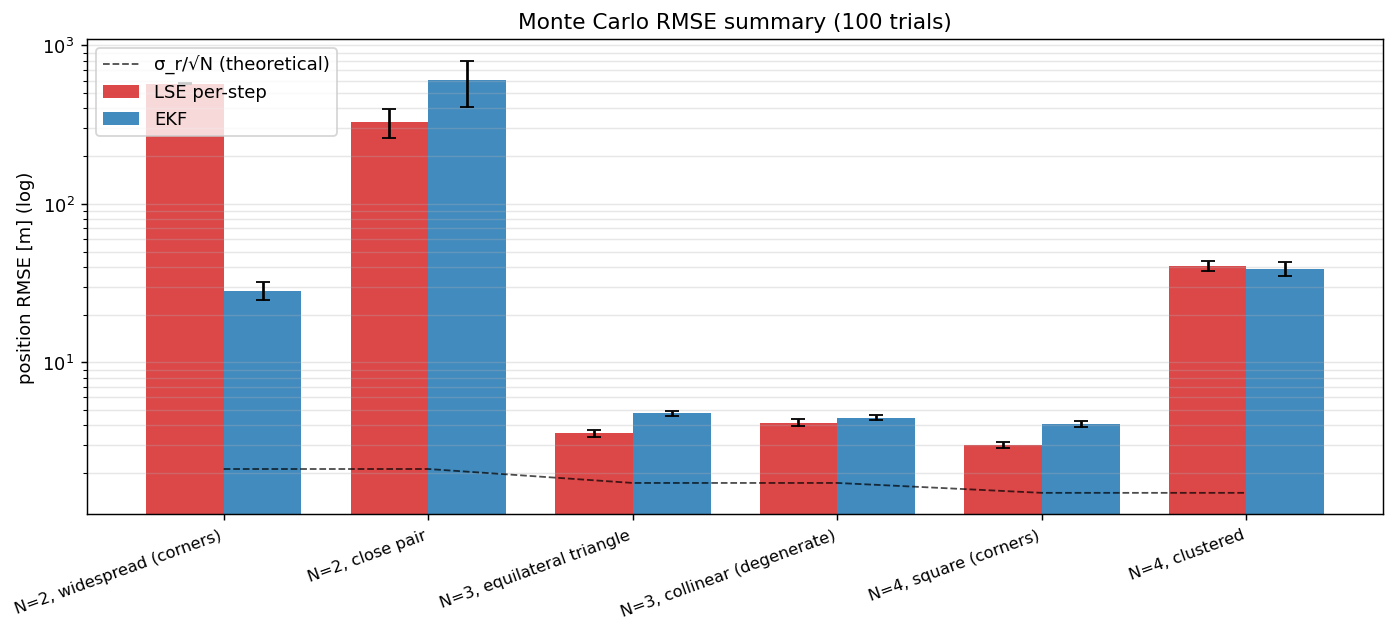
\includegraphics[width=\linewidth]{mc_rmse_summary.png}
  \caption{Overall RMSE; dashed line is $\sigma_r / \sqrt{N}$.}
\end{subfigure}\hfill
\begin{subfigure}{0.49\textwidth}
  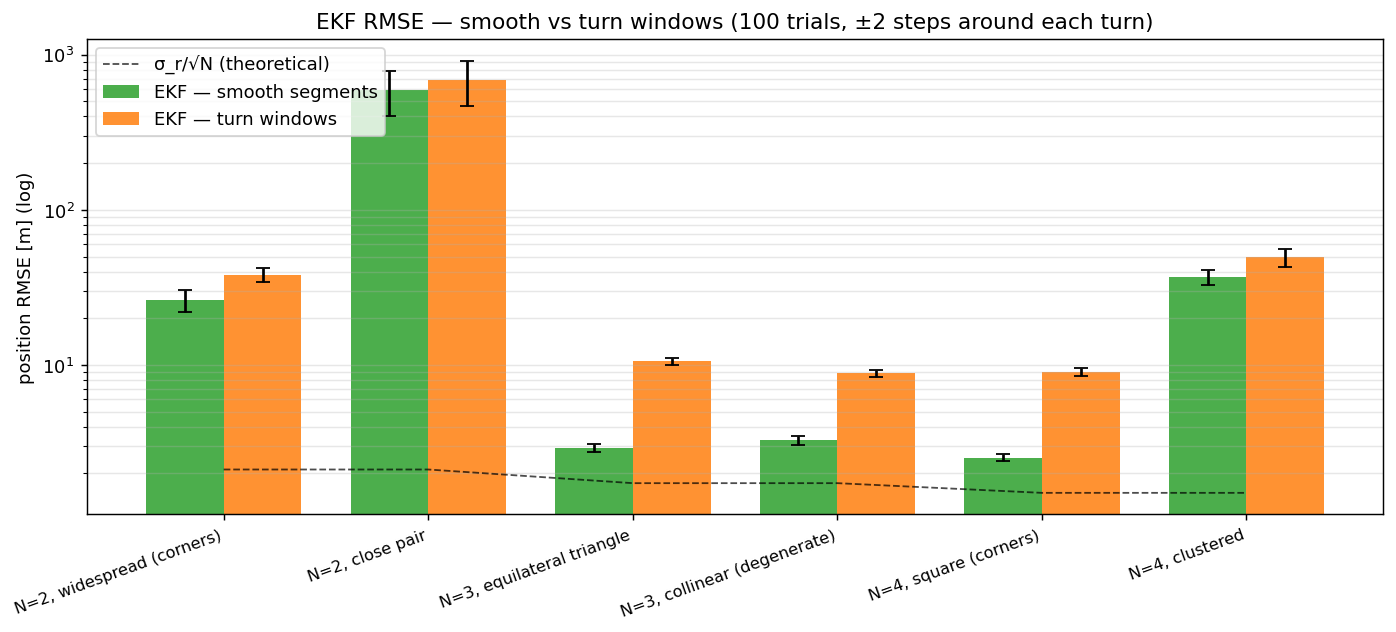
\includegraphics[width=\linewidth]{mc_rmse_smooth_vs_turn.png}
  \caption{EKF smooth vs.\ turn-window decomposition.}
\end{subfigure}
\caption{Monte Carlo RMSE summary across the six cells (100 trials each).}
\label{fig:mc-summary}
\end{figure}

The full per-cell error-vs-time panel grid (median and inter-quartile range
shading) is reproduced in Fig.~\ref{fig:mc-grid}; it shows the same story at
finer time resolution.

\begin{figure}[h]
\centering
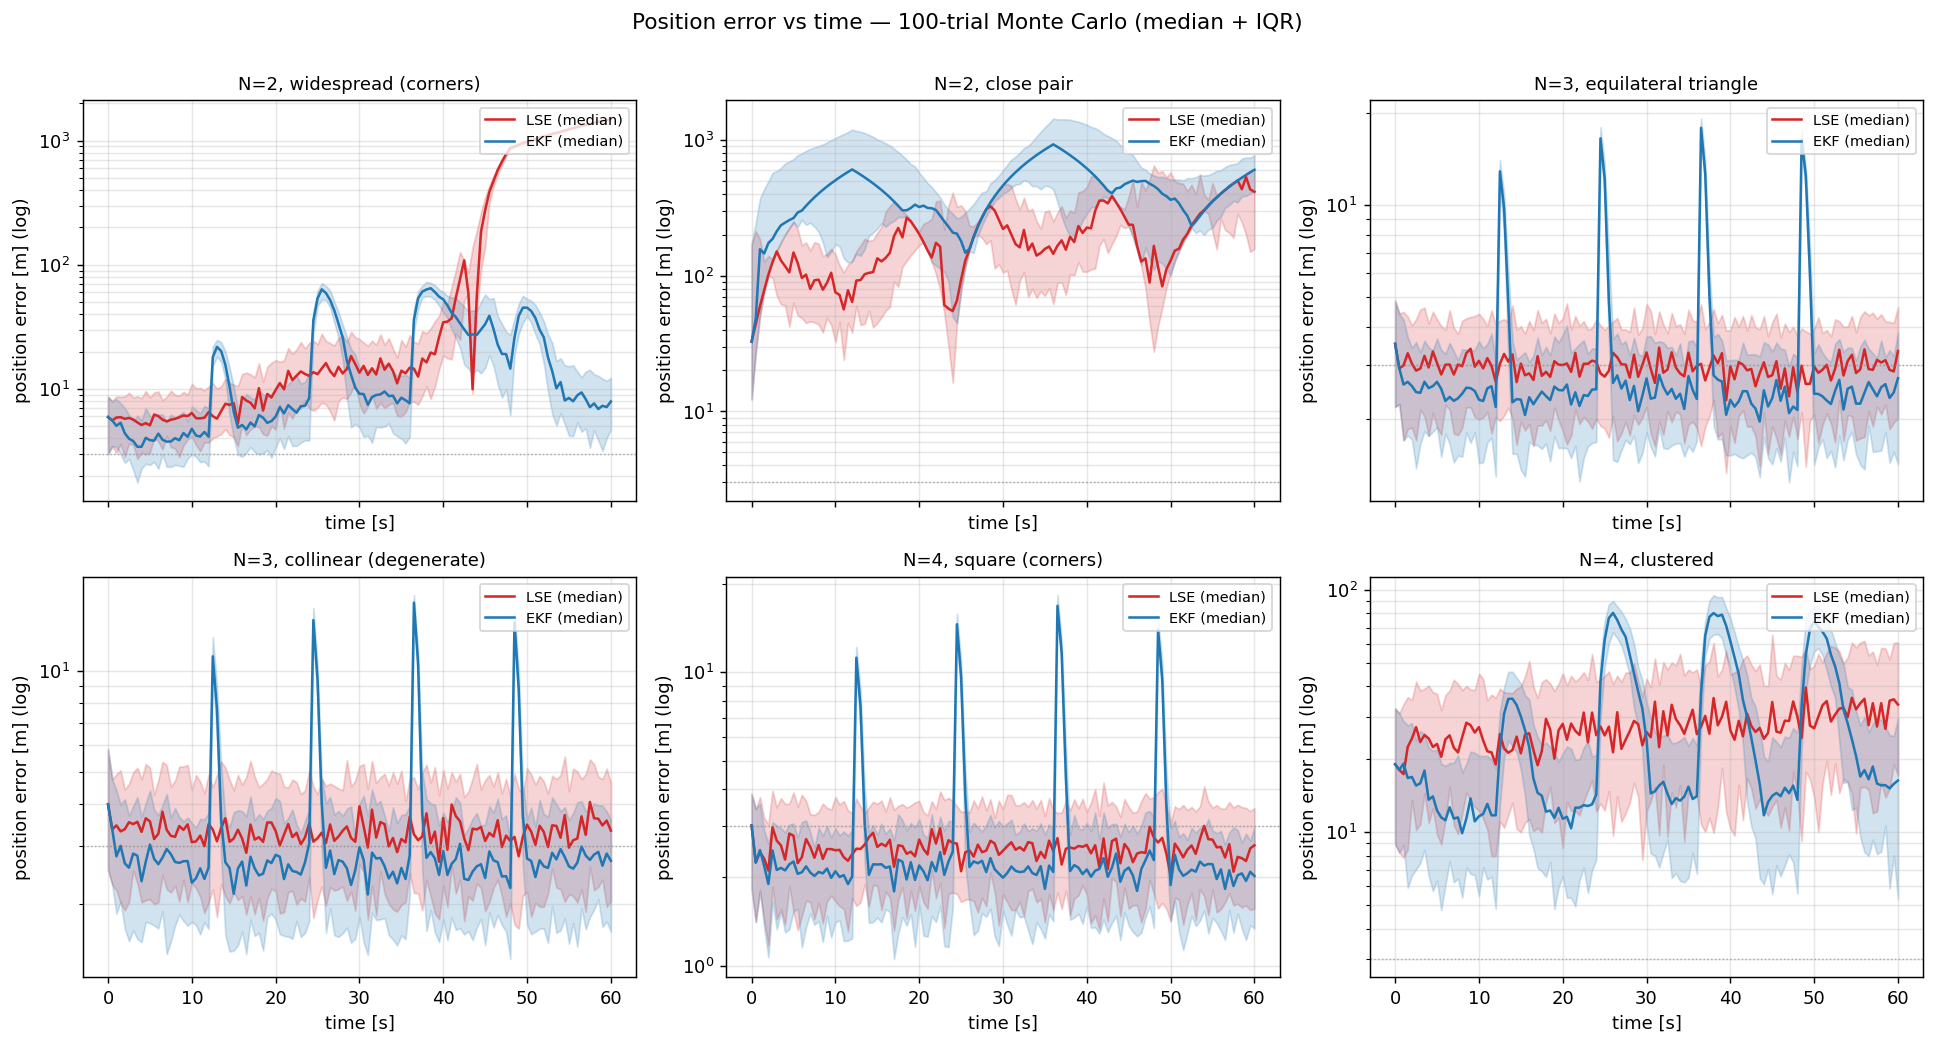
\includegraphics[width=0.95\textwidth]{mc_error_vs_time.png}
\caption{Position error versus time for each cell (100-trial Monte Carlo,
median curves and inter-quartile range).  Both estimators on log scale.}
\label{fig:mc-grid}
\end{figure}

\subsection{Smooth vs.\ Turn-Window Decomposition}
\label{sec:smooth-vs-turn}

The smooth-segment column of Table~\ref{tab:mc} confirms the expected
$\sigma_r / \sqrt{N}$ scaling for the well-conditioned cells: the
$N{=}4$ square cell achieves $2.52\,\mathrm{m}$ smooth-segment RMSE
against a theoretical bound of $1.5\,\mathrm{m}$, i.e.\ a factor of $1.7$.
The remaining gap is finite-filter overhead: the
$\mathbf{P}^{k|k}$ never reaches the asymptotic floor because the four
heading changes inject process noise at regular intervals.

The turn-window column tells a different story.  At $N{=}4$ square the EKF
RMSE during the post-turn transient is $9.07\,\mathrm{m}$, more than
three times the smooth-segment number and approximately the
prediction-error magnitude expected from a single-step lag:
$\norm{\mathbf{v}} \cdot T = 100 \cdot 0.5 = 50\,\mathrm{m}$ peak,
washing out over four steps to an averaged $\sim$$10\,\mathrm{m}$.
The turn-window error is therefore not random measurement noise; it is
deterministic prediction lag induced by a model mismatch (the CV model
does not know about the heading changes).

\subsection{Collinear Stress Test}
\label{sec:collinear}

The Monte Carlo summary in Table~\ref{tab:mc} shows the $N{=}3$
collinear cell tracking within $\sim$$1\,\mathrm{m}$ of the
$N{=}3$ equilateral triangle on every metric.  This is unexpected: for
sensors on the line $y=0$ the range measurements are invariant under the
reflection $(x, y) \mapsto (x, -y)$, so any candidate solution has a
mirror-image twin.  Why does the LSE/EKF pipeline not flip back and forth
between them?

Because the LSE warm-start prior $\mathbf{p}_{\text{prior}} = (3000,
4000)\,\mathrm{m}$ is on the same side of the sensor line as the true
trajectory, and the iterative Gauss-Newton converges to whichever side it
is initialised on.  Once the EKF is seeded, the velocity finite-difference
$\hat{\mathbf{v}}_0 = (\hat{\mathbf{p}}_1 - \hat{\mathbf{p}}_0)/T$
cements the correct branch, and there is no measurement-side information
that can distinguish the two solutions.

We confirm this experimentally by running the same configuration with three
priors:
%
\begin{table}[h]
\centering
\caption{Collinear $N{=}3$ stress test --- effect of LSE warm-start prior
(single deterministic run, seed $42$).}
\label{tab:collinear-stress}
\begin{tabular}{l r r}
\toprule
\textbf{Prior position} & \textbf{LSE RMSE [m]} & \textbf{EKF RMSE [m]} \\
\midrule
$(3000,\, 4000)$ \quad above (correct side)     & $3.89$        & $4.31$        \\
$(3000, -4000)$ \quad below (mirror image)      & $10\,763.05$  & $10\,763.11$  \\
$(5000,\, 0)$ \quad on the sensor line          & $5\,640.96$   & $5\,640.94$   \\
\bottomrule
\end{tabular}
\end{table}

\begin{figure}[h]
\centering
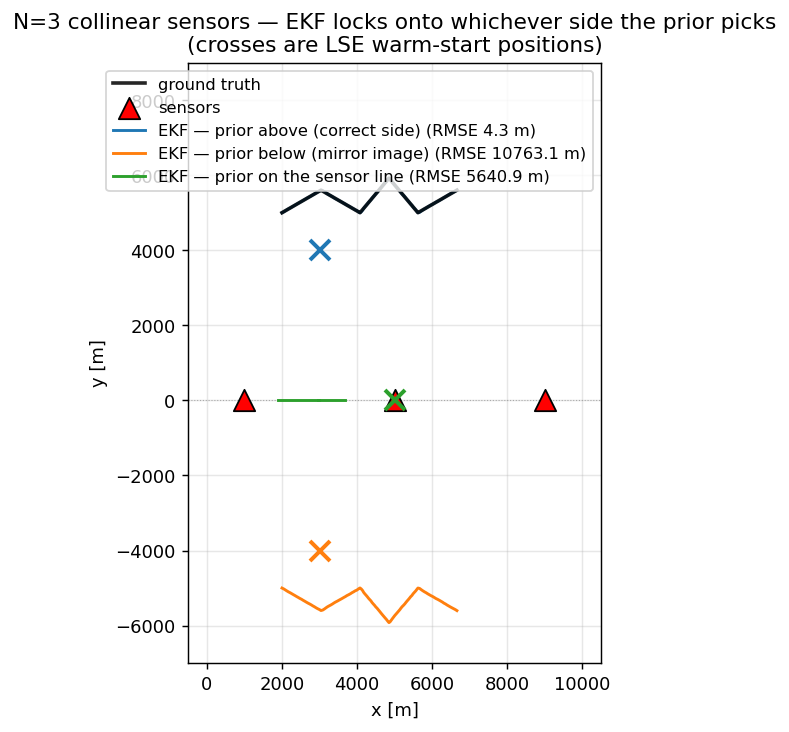
\includegraphics[width=0.85\textwidth]{collinear_stress.png}
\caption{Collinear $N{=}3$: the EKF tracks the same side of the sensor line
the prior was placed on; the on-line prior produces an unstable solution.
Crosses mark the LSE warm-start positions.}
\label{fig:collinear}
\end{figure}

The wrong-side prior produces an RMSE of about $10.7\,\mathrm{km}$, which
is essentially twice the average $y$-coordinate of the trajectory: the EKF
settles on a perfect mirror-image track and never escapes.  The on-line
prior produces $\sim 5.6\,\mathrm{km}$, half that number, because the LSE
picks each side stochastically.  The default
configuration's apparent robustness is therefore a feature of the prior,
not of the geometry: a real deployment would need either an unambiguous
prior (a fourth measurement, an asymmetric placement, or external
information) or a multi-hypothesis estimator.

\subsection{Process-Noise Sensitivity}
\label{sec:sigma-a-sweep}

Holding the geometry fixed at $N{=}4$ square, we sweep
$\sigma_a \in \{1, 5, 10, 50, 200\}\,\mathrm{m/s^2}$ with $30$ Monte Carlo
trials per setting.  Table~\ref{tab:sigma-a} and Fig.~\ref{fig:sigma-a}
report the smooth-segment and turn-window RMSE.

\begin{table}[h]
\centering
\caption{$\sigma_a$ sensitivity at $N{=}4$ square (30-trial MC).
The smooth-segment RMSE has a minimum near $\sigma_a = 10\,\mathrm{m/s^2}$;
the turn-window RMSE is monotone-decreasing in $\sigma_a$.}
\label{tab:sigma-a}
\begin{tabular}{r r r}
\toprule
$\sigma_a$ [m/s\textsuperscript{2}] & \textbf{Smooth RMSE [m]} & \textbf{Turn RMSE [m]} \\
\midrule
$1.0$    &  $22.68 \pm 0.21$ & $49.42 \pm 0.42$ \\
$5.0$    &   $2.72 \pm 0.16$ & $17.11 \pm 0.46$ \\
$10.0$   &   $2.55 \pm 0.16$ &  $8.98 \pm 0.46$ \\
$50.0$   &   $2.93 \pm 0.16$ &  $3.16 \pm 0.41$ \\
$200.0$  &   $3.02 \pm 0.17$ &  $2.94 \pm 0.38$ \\
\bottomrule
\end{tabular}
\end{table}

\begin{figure}[h]
\centering
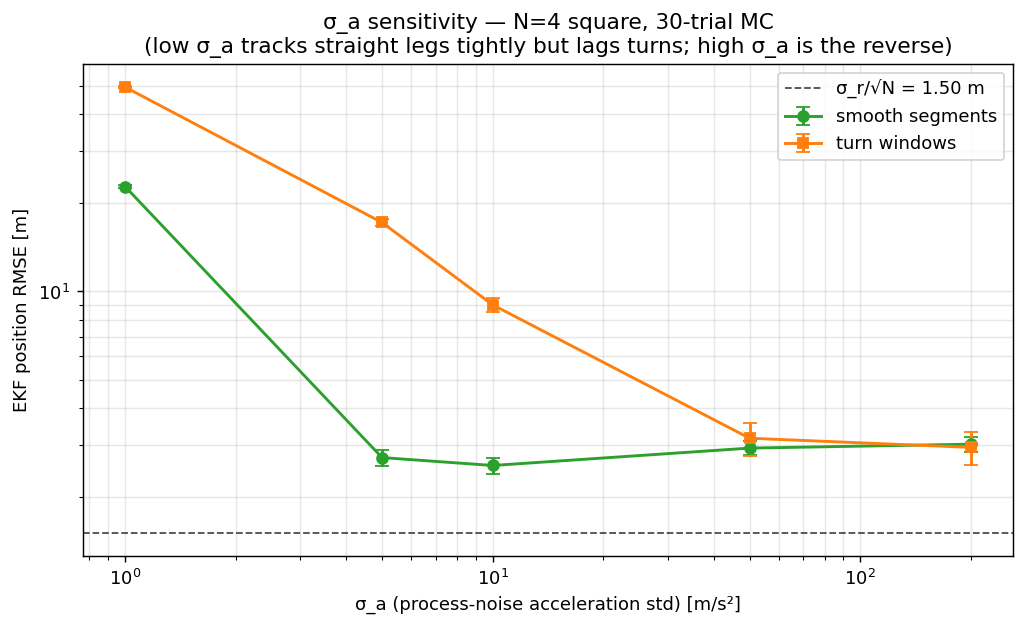
\includegraphics[width=0.7\textwidth]{sigma_a_sweep.png}
\caption{$\sigma_a$ sensitivity sweep, $N{=}4$ square.  Low $\sigma_a$ --
the filter is too rigid and accumulates lag during turns.  High $\sigma_a$
-- the filter trusts measurements over the velocity model, so turns recover
quickly but baseline noise creeps up.  The default $\sigma_a = 10$ is at a
reasonable knee on the smooth side.}
\label{fig:sigma-a}
\end{figure}

The trade-off is monotonic and resolves the choice of $\sigma_a$ as a
single-axis design decision: at $\sigma_a = 1\,\mathrm{m/s^2}$ the filter
cannot keep up with the maneuvers and accumulates $> 20\,\mathrm{m}$ error
even on smooth segments; at $\sigma_a = 200\,\mathrm{m/s^2}$ it
essentially reduces to an instantaneous LSE plus a small Bayesian
smoothing prior.  No single $\sigma_a$ minimizes both columns; if turn
responsiveness is preferred over smooth-segment precision, $\sigma_a \in
[50, 100]$ would be a better operating point than the default.

% =============================================================================
\section{Discussion}
\label{sec:discussion}

\subsection{The Geometry Story}

The Monte Carlo summary cleanly separates three failure modes:
%
\begin{enumerate}[leftmargin=2em]
  \item \textbf{Pure geometric dilution} (\texttt{N4\_cluster},
        \texttt{N2\_close}): when the unit vectors $\mathbf{u}_i$
        in~\eqref{eq:H-rows} span a small angle, the matrix
        $\mathbf{H}\transpose \mathbf{H}$ is poorly conditioned and the
        position covariance~\eqref{eq:Pp} is large.  The $N{=}4$
        clustered configuration delivers $\sim$$37\,\mathrm{m}$ smooth
        RMSE despite the same $\sigma_r$ and the same $N$ as the square
        cell --- a tenfold penalty traceable entirely to GDOP.
  \item \textbf{Estimator ambiguity} (\texttt{N2\_close},
        \texttt{N3\_collinear} with wrong prior): with insufficient or
        symmetric geometry, the range constraints permit multiple
        solutions and the estimator picks one based on side information.
        This produces dramatic, prior-dependent failure modes that
        \emph{cannot} be diagnosed from the per-cell smooth RMSE alone.
  \item \textbf{Model mismatch} (every cell, during turns): the CV
        motion model does not know about the heading changes, so a
        prediction error of $\sim$$\norm{\mathbf{v}} T = 50\,\mathrm{m}$
        appears at each turn and washes out over a few steps.  The
        averaged turn-window RMSE for well-conditioned cells is
        $\sim$$9\,\mathrm{m}$, four times the smooth-segment number.
\end{enumerate}

\subsection{LSE vs.\ EKF}

A non-obvious finding is that the per-step LSE matches or slightly beats
the EKF on \emph{overall} RMSE in the well-conditioned cells.  This is not
an indictment of the EKF; it is a consequence of how the two estimators
interact with the trajectory.  The EKF's smoothing benefit is concentrated
in the smooth segments (where it gains roughly $\sigma_r$ versus
per-step LSE), while its lag cost is concentrated in the turn windows
(where it loses $\sim$$5\,\mathrm{m}$ versus an instantaneous estimator).
With four turns over a $60\,\mathrm{s}$ trajectory, the lag cost
dominates the smooth gain in the blended RMSE.  When the per-step
estimator is fragile (\texttt{N2\_wide}, where two-circle ambiguity
produces large outliers), the EKF's prior smooths the outliers and it
wins decisively: $28\,\mathrm{m}$ versus $573\,\mathrm{m}$.

The right metric is therefore the \emph{decomposed} RMSE, not the blended
one.  On smooth segments the EKF beats per-step LSE in every well-conditioned
cell; on turn windows neither estimator distinguishes itself, which is
the cue for a more capable motion model.

\subsection{Limitations and Future Work}

\paragraph{Motion model.}
The CV model is the obvious bottleneck.  An Interacting Multiple Model
(IMM) filter mixing CV with a coordinated-turn (CT) model would close
most of the turn-window gap.  The course spec deliberately scopes this
out, but the data here motivates it cleanly.

\paragraph{Measurement model.}
The TOA model assumes synchronized sensors and known emission times.  TDOA
relaxes the second requirement at the cost of a pairwise differencing step
and a slightly higher effective noise floor; it is an alternative the
spec also allows and is a natural extension.

\paragraph{Theoretical bound.}
The smooth-segment RMSE sits at $\sim$$1.7\sigma_r/\sqrt{N}$ for the
square cell.  Computing the exact Cram\'er--Rao lower bound for the
position estimator would quantify how far above the bound the EKF
operates and is straightforward given~\eqref{eq:Pp}.

\paragraph{Beyond the prior.}
The collinear ambiguity result suggests adding a multi-hypothesis tracker
(Gaussian-Mixture or Particle Filter) for the truly ambiguous geometries.
A two-hypothesis EKF that tracks both $\pm y$ branches and uses any
asymmetry-breaking measurement to weight them would be a small extension.

% =============================================================================
\section{Conclusion}

A modest pipeline --- TOA simulation, Gauss-Newton LSE initialization, and
a constant-velocity EKF --- recovers position to within $1.7\sigma_r/\sqrt{N}$
on smooth segments at a well-placed four-sensor geometry, and degrades
predictably under three identifiable failure modes: GDOP (cluster /
close-pair), estimator ambiguity (collinear / two-sensor), and motion-model
mismatch (the four heading changes).  The decomposed RMSE metric is essential
for isolating which mode is dominant in any given cell.  Of the analyses
performed, the collinear stress test is the most pedagogically valuable: it
shows that an apparently well-behaved geometry can hide a fundamental
degeneracy that the prior is silently absorbing.  The next step in the same
spirit would be an IMM filter --- the data already shows where it would help.

% =============================================================================
\section*{Code and Reproducibility}

All experiments in this report can be reproduced from the public
repository at
\url{https://github.com/selcuko/mth407-toa-target-tracking}.
Running \texttt{python main.py --no-anim} produces every figure and CSV
referenced here in under a minute.  Random seeds are fixed in each
experiment script so results are bit-exact across runs.

\end{document}
